\documentclass[11pt]{article}
 \renewcommand{\familydefault}{\sfdefault}

 \usepackage{xcolor}
 % Define custom colors for code highlighting
\definecolor{cppkeyword}{RGB}{0,0,255} % Blue
\definecolor{cppcomment}{RGB}{0,128,0} % Green
\definecolor{cppstring}{RGB}{255,0,0} % Red

\usepackage{listings}
\lstset { %
    language=C++,
    %backgroundcolor=\color{blue}, % set backgroundcolor
	basicstyle=\ttfamily\color{black}, % Regular font style
    commentstyle=\color{cppcomment}, % Set the color for comments
    keywordstyle=\bfseries\color{cppkeyword}, % Set the color for keywords
    stringstyle=\color{cppstring}, % Set the color for strings
    numbers=left, % Display line numbers
    numberstyle=\tiny\color{gray}, % Line number font style
    stepnumber=1, % Line numbers increment by 1
    tabsize=2, % Tab size
    rulecolor=\color{black}, % Frame color}
}

\title{Relazione progetto di Programmazione ad Oggetti}
\author{Carlo Rosso}

\usepackage{comment}
\usepackage{tabularx}
\usepackage{changepage}
\usepackage{amsfonts}
\usepackage{float}
\usepackage{amsmath}
\usepackage{graphicx}
\usepackage{hyperref}
\usepackage{caption}
\usepackage{fancyhdr}
\usepackage{adjustbox}
\usepackage{geometry}
	\geometry{height=24 cm}
	\geometry{left=2.5 cm}
	\geometry{right=2.5 cm}
	\geometry{top=2 cm}
	\geometry{headheight=1 cm}

\setcounter{secnumdepth}{0}
\linespread{1}
\renewcommand{\labelitemi}{-}
\newtheorem{definition}{Def.}[section]
\newtheorem{theorem}{Teorema}[section]
\newtheorem{proof}{Dimostrazione}[section]


\begin{document}

\section{Music vs Robots}

\begin{table}[ht]
	\begin{tabular}{|l|l|l|}
		\hline
		\textbf{Cognome} & \textbf{Nome} & \textbf{Matricola} \\ \hline
		Pellegrinelli & Nicolò & 2034334 \\ \hline
		Rosso & Carlo & 2034293 \\ \hline
	\end{tabular}
\end{table}

"Music vs Robots" è un programma scritto interamente in c++ che si ispira al 
famoso gioco mobile Plants vs Zombie.
Il gioco si basa su una griglia, chiamata Game, in cui si possono 
inserire, rimuovere e migliorare degli strumenti musicali (copia delle piante) 
che suonano per sconfiggere i robot (zombie) che arrivano dal lato destro.
L’obiettivo del gioco è quello di resistere il più possibile all’attacco dei 
robot. Il gioco termina se almeno un robot raggiunge il lato sinistro del 
Playground.
La scelta iniziale è stata da subito molto combattuta: l’obiettivo era 
realizzare un programma interessante e sfidante ma allo stesso tempo gradevole
da sviluppare.
La scelta si è rivelata soddisfacente e divertente. Lo sviluppo è stato
estenuante in alcuni punti, ma siamo riusciti a portare a termina il progetto
rispettando le nostre aspettative.

\subsection{Descrizone del modello}

Il modello si suddivide in due parti:
\begin{itemize}
	\item La gestione delle entità del gioco, ovvero i robot e gli strumenti
		musicali che producono i danni;

	\item La gestione del gioco, ovvero la griglia in cui si muovono le entità
		e la gestione del tempo e l'aumento della difficoltà ad esso legato.
\end{itemize}

\subsubsection{Gestione delle entità}
\begin{figure}[ht]
	\centering
	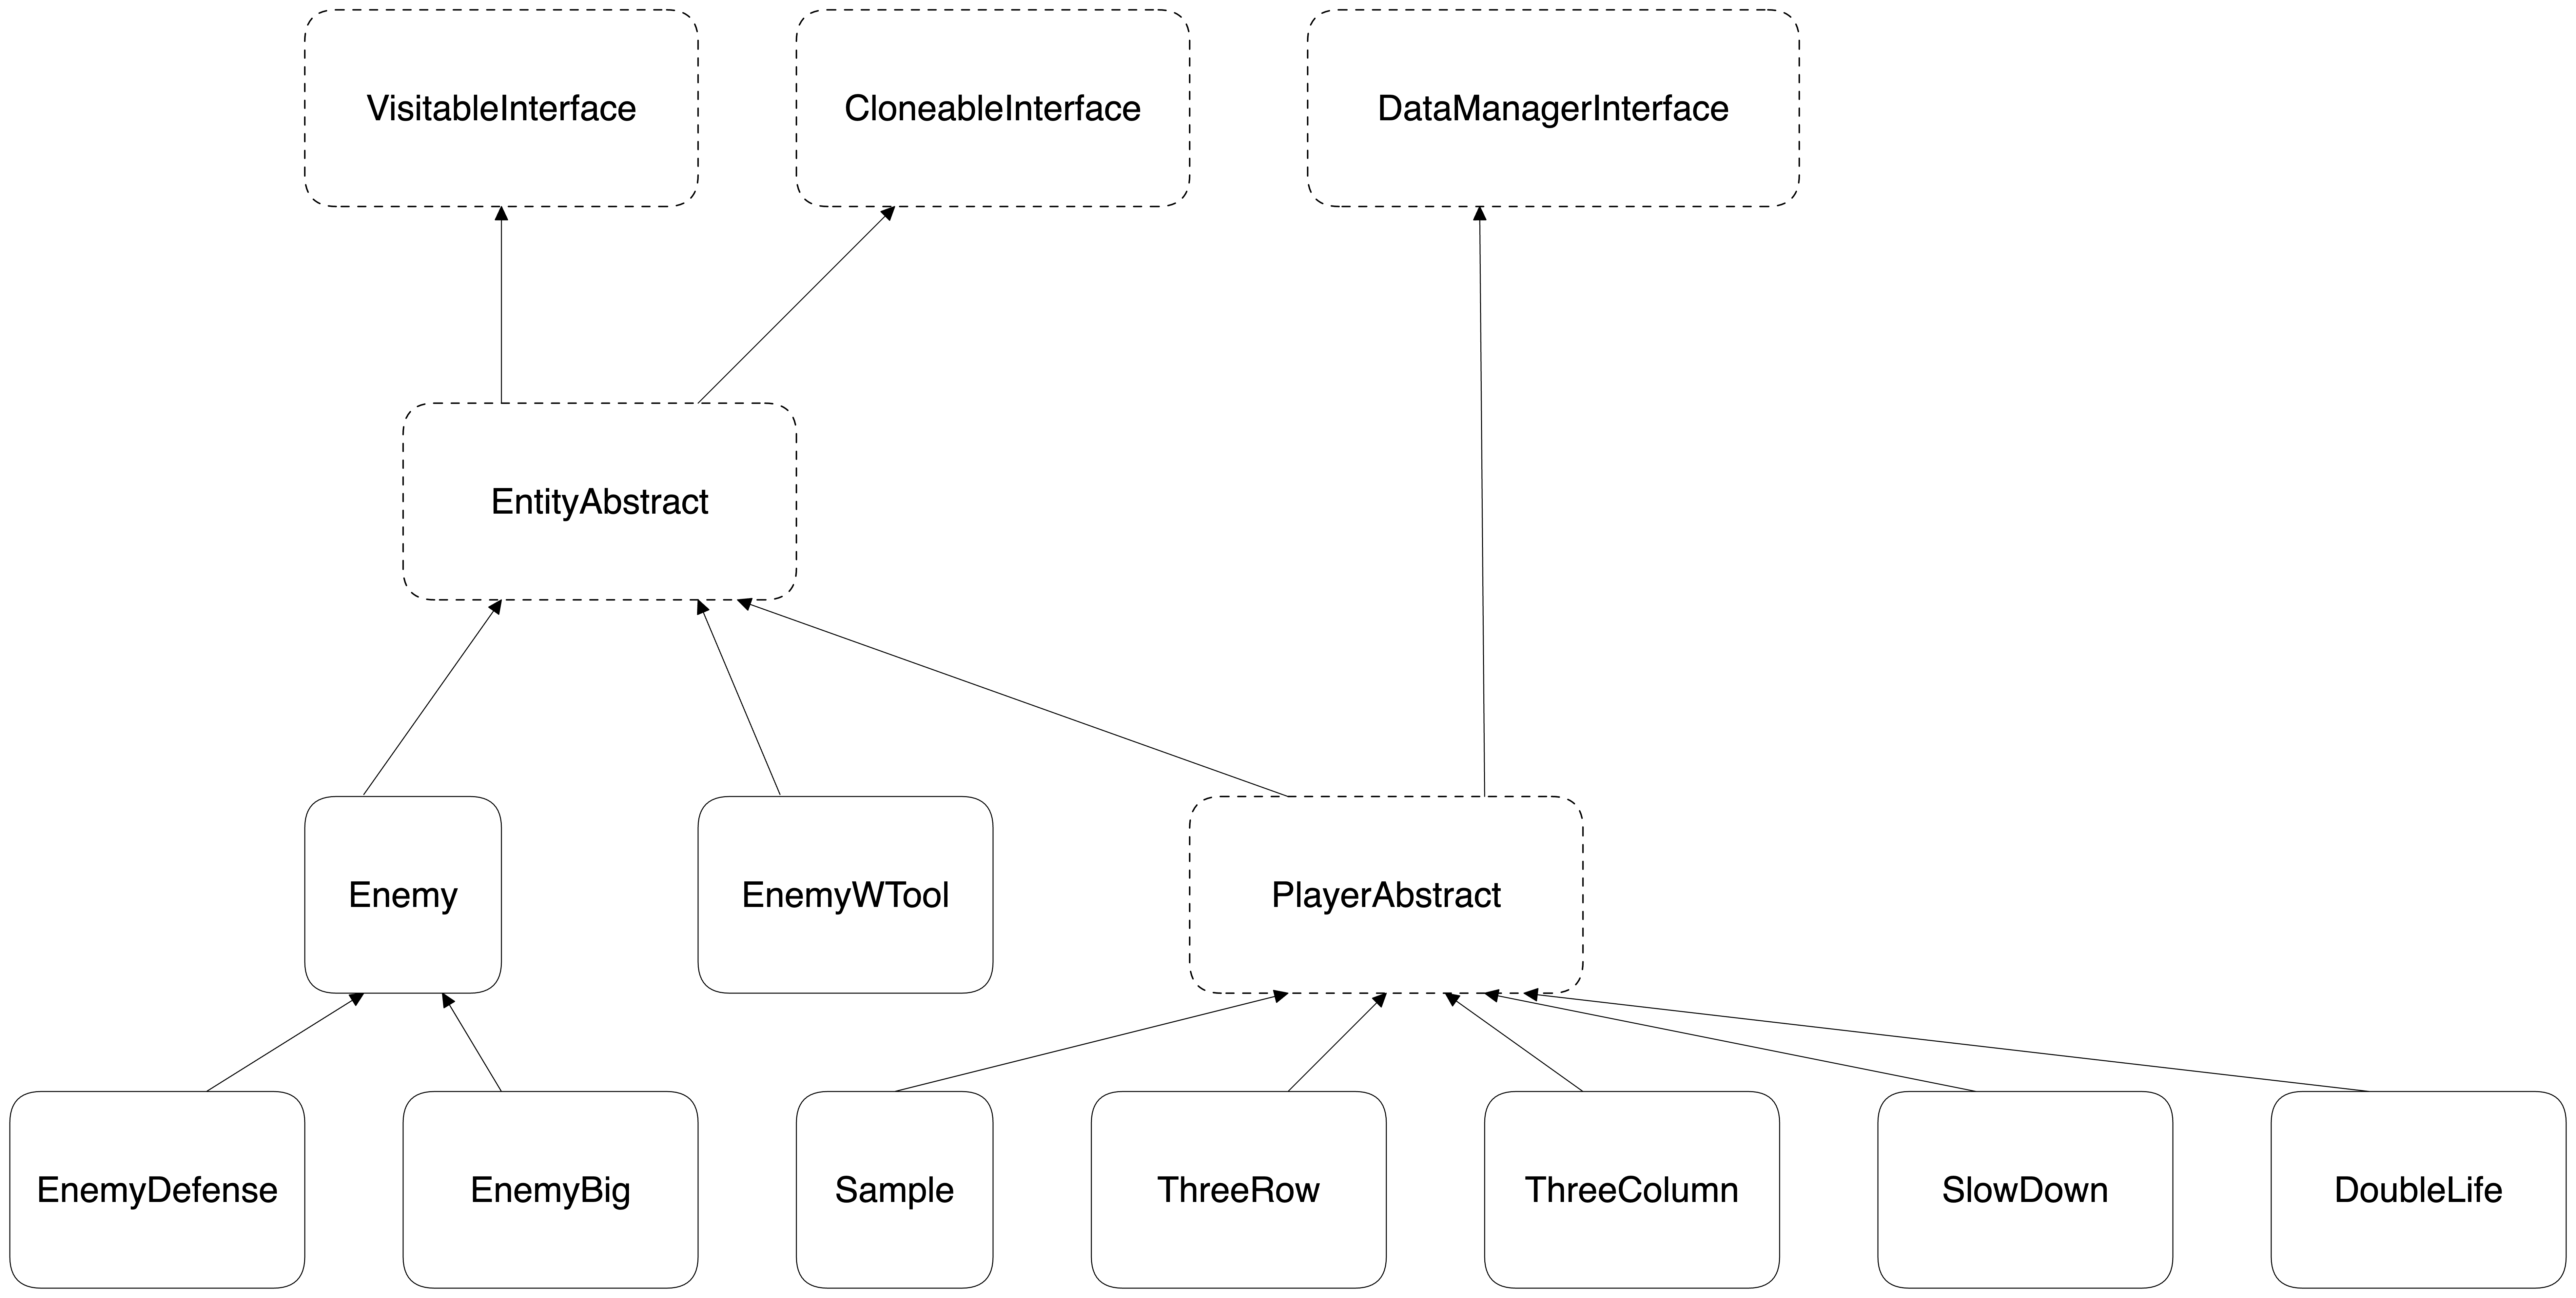
\includegraphics[width=\textwidth]{assets/entity}
	\caption{Gerarchia delle entità}
\end{figure}

La gerarchia comincia con tre classi astratte:
\begin{itemize}
	\item VisitableInterface: interfaccia che permette di visitare un oggetto
		mediante il pattern Visitor, attraverso il metodo accept. Questa classe
		è utilizzata dalla classe VisitorInterface per accedere alle immagini 
		delle entità;

	\item CloneableInterface: interfaccia che permette di clonare un oggetto
		mediante il pattern Prototype, attraverso il metodo clone. Per esempio,
		abbiamo definito una classe \lstinline|ptr<T>|, si tratta di uno smart pointer
		classico, con l'aggiunta che la classe T deve implementare
		CloneableInterface;

	\item DataManagerInterface: tutti gli oggetti che implementano questa
		interfaccia possono essere salvati e caricati da un file;
\end{itemize}

Le prime due classi sono ereditate da EntityAbstract, una classe astratta 
che gestisce le interzioni tra le entità. Le entità possono effettuare due 
azioni principali: possono attaccare e ricevere danno. \\
Le classi che ereditano da EntityAbstract sono:
\begin{itemize}
	\item PlayerAbstract: è una classe astratta perché non implementa alcuni
		metodi delle interfacce e della classe EntityAbstract; inoltre definisce
		metodi virtuali puri che devono essere implementati dalle classi che
		ereditano da essa. Le classi che derivano da PlayerAbstract sono gli
		strumenti musicali che sono utilizzati per difendersi dai robot;

	\item Enemy: è una classe concreta che rappresenta i robot che attaccano
		l'utente. Questa classe rappresenta il robot più semplice. Da Enemy
		derivano le classi EnemyDefense e EnemyBig che rappresentano dei robot
		con caratteristiche diverse;

	\item EnemyWTool: utilizza la relazione "has-a" e
		rappresenta un robot con un Tool. I tool migiorano qualche proprietà del 
		robot. Enemy e tool sono generati casualmente utilizzando il pattern
		Factory;
\end{itemize}

Le entità interagiscono tra di loro generando i danni o subendoli.

\begin{figure}[ht]
	\centering
	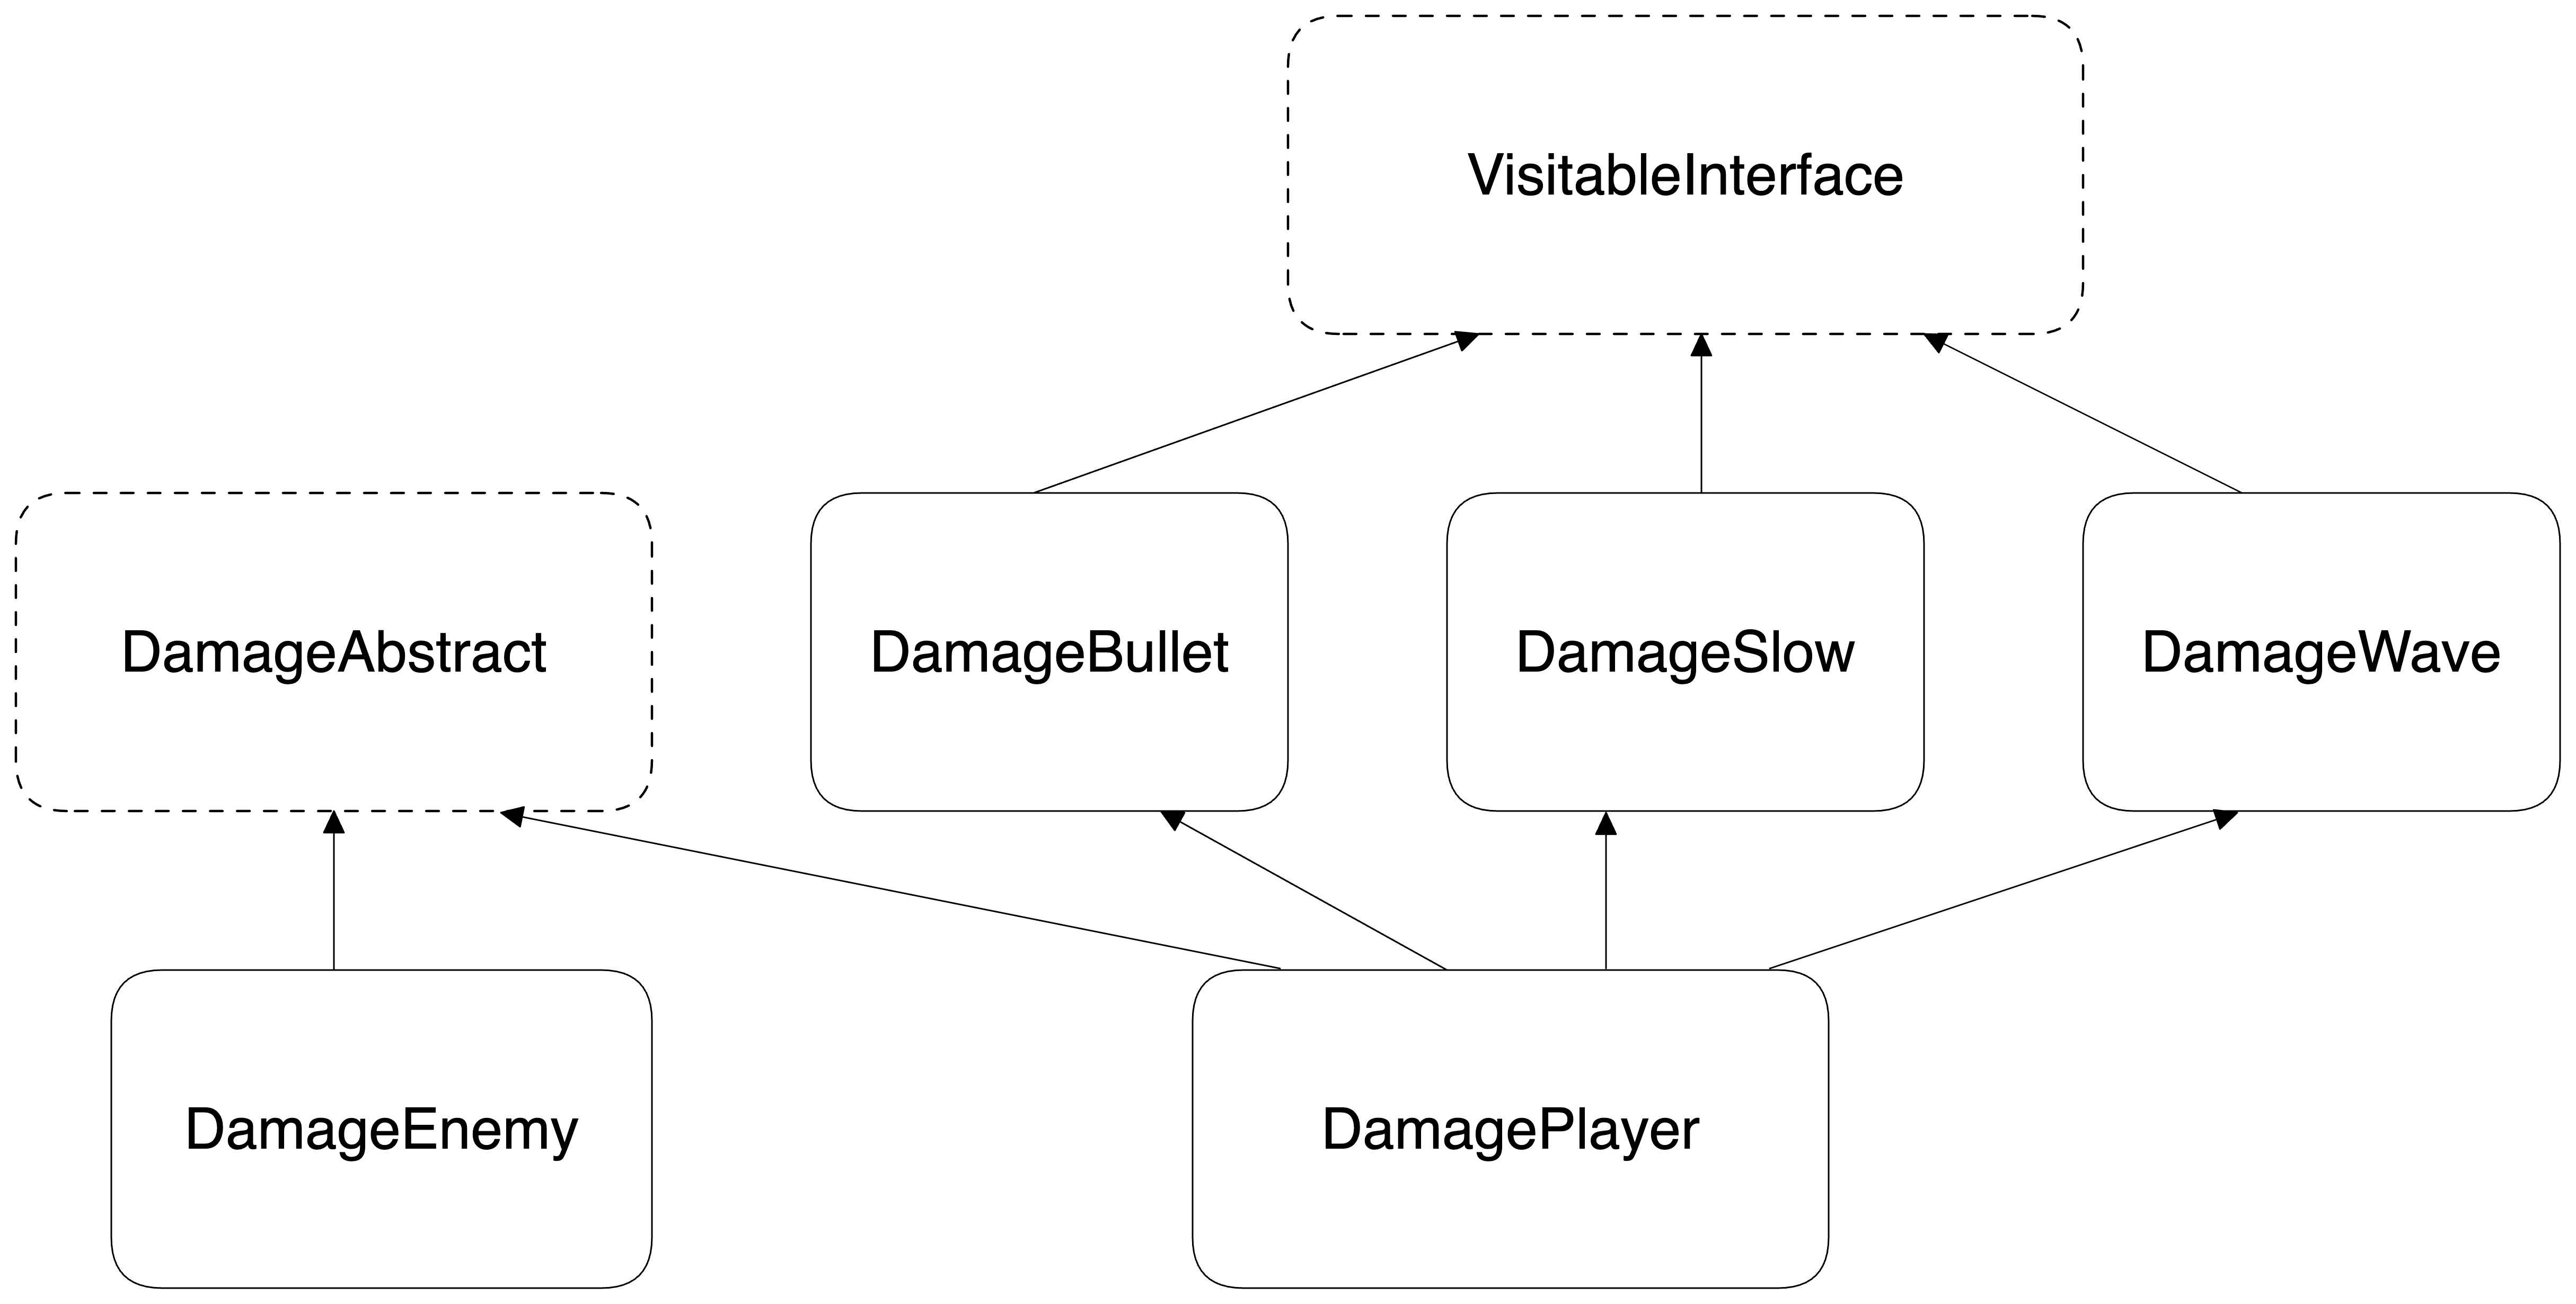
\includegraphics[scale = 0.05]{assets/damage}
	\caption{Gerarchia dei danni}
\end{figure}

La classe DamageEnemy rappresenta i danni che sono generati dai robot e sono
inflitti agli strumenti musicali. \\
La classe DamagePlayer rappresenta i danni che sono generati dagli strumenti
musicali e sono inflitti ai robot. Eredita da VisitableInterface perché
sono visibili. Eredita da tre classi concrete, anche se non sono mai istanziate
singolarmente, perché gli strumenti musicali possono generare diversi tipi di
danni. DamageBullet rappresenta i danni che si infrangono sul primo robot;
DamageSlow non infligge alcun danno, ma rallenta i robot; DamageWave infligge la
stessa quantità di danno su tutti i robot per un certo numero di colonne.

\subsubsection{Gestione del gioco}

\begin{figure}[ht]
	\centering
	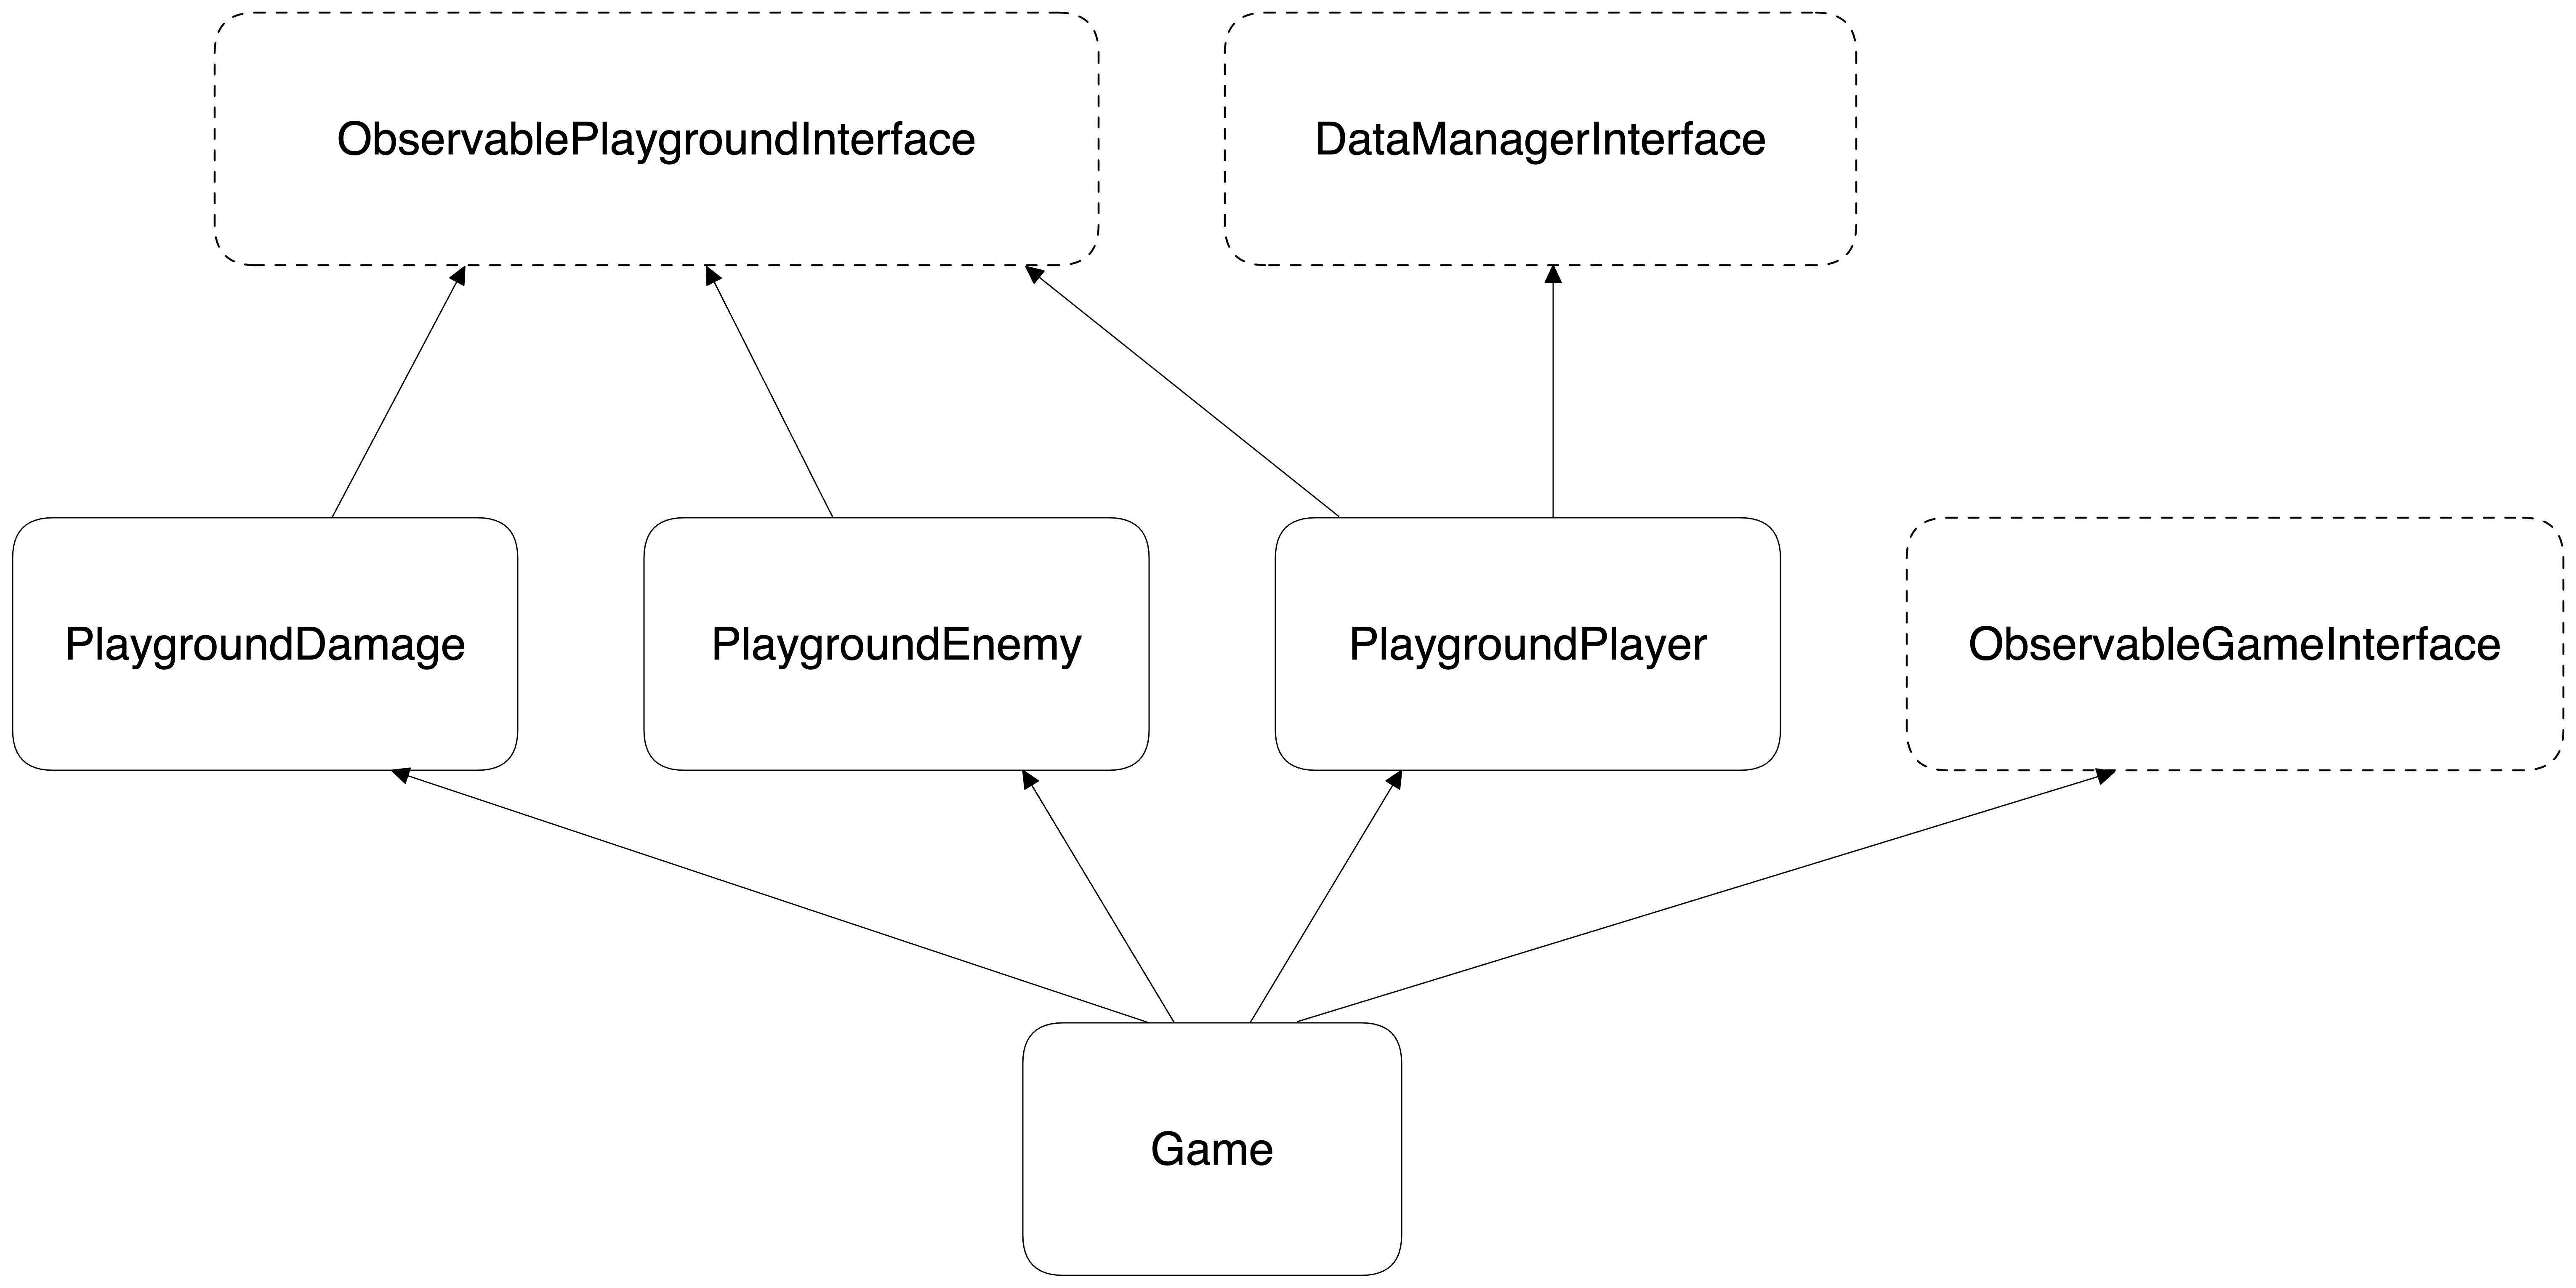
\includegraphics[scale=0.045]{assets/game}
	\caption{Gerarchia del gioco}
\end{figure}

ObservablePlaygroundInterface è l'interfaccia utilizzata per comunicare alla
grafica le modifiche che avvengono nel gioco. \\
Ci sono tre classi da cui eredita Game oltre a ObservableGame:
\begin{itemize}
	\item PlaygroundPlayer: è composta da una griglia di 
		\lstinline|ptr<PlayerAbstract>|. Questa classe gestisce gli strumenti 
		musicali che attaccano i robot;
		 
	\item PlaygroundEnemy: è composta da una griglia di 
		\lstinline|deque<EnemyWTool>|, perchè ci possono essere più robot sulla 
		stessa cella. 
		Questa classe gestisce i robot che attaccano gli strumenti musicali;

	\item PlaygroundDamage: è composta da una griglia di 
		\lstinline|ptr<DamagePlayer>|. 
		Questa classe gestisce i danni che sono generati dagli strumenti 
		musicali e sono inflitti ai robot;
\end{itemize}
La classe Game gestisce le interazioni tra le tre classi Playground e sfrutta il
pattern Singleton per mantenere un'unica istanza del gioco accessibile da
qualsiasi punto del programma.

\subsection{Utilizzo del polimorfismo}

Il polimorfismo è stato utilizzato in EnemyWTool, per quanto riguarda le entità.
Infatti i vari robot ed i vari tool sono gestiti in modo interscabiabile dalla 
classe EnemyWTool.\\
Il polimorfismo è sfruttato in modo più ampio nella gestione del gioco. Infatti,
la classe Game gestisce le interazioni tra le entità utilizzando i metodi
virtuali puri definiti in EntityAbstact e in PlayerAbstract. 
Le principali funzioni virtuali della gerarchia sono:
\begin{itemize}
	\item \lstinline|bool sufferDamage(DamageAbstract &damage)|: questa funzione 
		viene chiamata quando un'entità subisce un danno. Ritorna true se 
		l'entità è stata distrutta, false altrimenti;

	\item \lstinline|DamageAbstract *attack() const|: questa funzione viene chiamata quando
		un'entità attacca. Ritorna un puntatore al danno che viene generato
		dall'entità;

	\item \lstinline|CloneableInterface *clone() const|;

	\item \lstinline|void accept(VisitorInterface &visitor) const|: il metodo è
		utilizzato per accedere ad un istanza di VisitableInterface. È chiamato
		da VisitorInterface, in particolare da imageVisitor, per accedere
		all'immagine dell'entità;


	\item \lstinline|void levelUp()|: viene utilizzata per aumentare il livello 
		di uno struemnto musicale;

	\item \lstinline|u32 getCost()|: ritorna il costo per posizionare uno strumento musicale
		sulla griglia, oppure il costo per effettuare l'upgrade di uno
		strumento musicale già presente sulla griglia;

	\item \lstinline|u32 move()|: ritorna il numero di celle che uno robot può 
		percorrere in un turno;

	\item \lstinline|u32 damage()|: ritorna il danno che un oggetto 
		DamageAbstract infligge;

	\item \lstinline|bool slow()|: ritorna true se un oggetto DamagePlayer rallenta gli
		EnemyWTool, false altrimenti;

	\item \lstinline|void oneWave()|: indica all'oggetto DamagePlayer che ha percorso una
		cella.
\end{itemize}



\subsection{Persistenza dei dati}

La persistenza dei dati è gestita attraverso la classe DataManagerInterface.
Infatti, tutte le classi che devono essere salvate o caricate da un file JSON
ereditano da essa; ovvero: PlayerAbstract, PlaygroundPlayer, Cash e Timer.
Le classi che ereditano da DataManagerInterface devono implementare i seguenti
metodi:
\begin{itemize}
	\item \lstinline|std::string toString() const|: viene utilizzata per 
		convertire la classe in una stringa, in modo da poterla salvare su un 
		file;

	\item \lstinline|DataManagerInterface *fromString(std::string)|: viene 
		utilizzata per convertire una stringa in una classe, in modo da poterla 
		caricare da un file;
\end{itemize}

Il metodo \lstinline|static void saveAll()| viene invocato alla chiusura del 
programma o al ritorno alla schermata principale e chiama il metodo
\lstinline|std::string toString() const| su tutti
gli oggetti che sono da salvare. Il metodo \lstinline|static bool loadAll()| 
viene invocato per caricare l'ultima partita salvata, sfruttando i metodi 
\lstinline|DataManagerInterface *fromString(std::string)|. Il file example.json 
contiene un esempio di salvataggio.

\subsection{Funzionalità implementate}

\begin{itemize}
	\item Inserimento di strumenti musicali sulla griglia;

	\item Rimozione di strumenti musicali dalla griglia;

	\item Upgrade di strumenti musicali;

	\item Visualizzazione del livello degli strumenti musicali;

	\item Inserimento di un robot sulla griglia ad ogni clock. Con relativo
		aumento dell'attacco e della vita in funzione del tempo;

	\item Salvataggio automatico delle partite e caricamento dell'ultima
		partita salvata;

	\item Visualizzazione del tempo dall'inizio della partita;

	\item Visualizzazione del denaro disponibile e del costo di inserimento di
		uno strumento musicale o del suo upgrade;

	\item Movimento dei robot verso gli strumenti musicali;

	\item Inserimento dei danni generati dagli strumenti musicali; 
	
	\item Movimento dei danni;

	\item Utilizzo di immagini per visualizzare gli strumenti musicali, i robot
		e i danni;
\end{itemize}

\subsection{Rendicontazione delle ore di lavoro}

\begin{table}[H]
	\centering
	\begin{tabular}{|l|l|l|}
		\hline
		\textbf{Attività} & \textbf{Ore Previste} & \textbf{Ore Effettive} \\
		\hline
		Progettazione & 10 & 17 \\
		\hline
		Sviluppo del codice del modello & 25 & 45 \\
		\hline
		Studio del framework Qt & 5 & 5 \\
		\hline
		Sviluppo del codice della GUI & 5 & 5 \\
		\hline
		Test e debug & 10 & 25 \\
		\hline
		Stesura della relazione & 5 & 3 \\
		\hline
		\textbf{Totale} & \textbf{60} & \textbf{100} \\
		\hline
	\end{tabular}
\end{table}

Le ore effettive sono state maggiori di quelle previste, perché siamo incorsi in
un bug che non siamo riusciti a risolvere. Tutt'ora rimango all'oscuro del
problema che si verificava. Le ore di debug sono molto maggiori delle 
aspettative proprio per questo motivo. Dopo diversi tentativi di risoluzione 
del problema,
abbiamo deciso di riscrivere la logica del gioco. In effeti, credevo che la
riscrittura sarebbe stata piuttosto lenta. Al contrario, avendo già un esempio
da seguire si è rivelata piuttosto rapida; anzi ci ha dato modo di riorganizzare
il codice per mostrare più chiaramente i pattern implementati. Inoltre,
l'implementazione dei danni è potuta partire dal basso.

\subsection{Suddivisione delle attività}

\begin{table}[H]
	\centering
	\begin{tabular}{|l|l|}
		\hline
		\textbf{Attività} & \textbf{Sviluppatore} \\
		\hline
		Implementazione di EnemyWTool e derivati & Carlo \\ \hline
		Implementazione di PlayerAbstract e derivati & Nicolò \\ \hline
		Sviluppo di DamageAbstract e derivati & Nicolò \\ \hline
		Sviluppo di PlaygroundPlayer e PlaygroundEnemy & Carlo \\ \hline
		Sviluppo di PlaygroundDamage & Nicolò \\ \hline
		Sviluppo di Cash e Timer & Tutti \\ \hline
		Sviluppo di Game & Tutti \\ \hline
		Sviluppo dell'utilità & Tutti \\ \hline
		Sviluppo della GUI & Tutti \\ \hline
		Salvataggio su file & Carlo \\ \hline
		Caricamento da file & Nicolò \\ \hline
	\end{tabular}
\end{table}

\subsection{Considerazioni finali}

Abbiamo scelto un progetto che ci permettesse di sperimentare quanto più
possibile ciò che abbiamo imparato in questi anni di università. Ci siamo 
cimentati in un'applicazione più ampia di quanto effetivamente
richiesto, perché siamo appassionati alla programmazione, in primo luogo; 
inoltre
è nostro interesse arricchire il nostro portfolio per
dimostrare le nostre capacità, alcune cose che abbiamo imparato e la nostra
passione per la programmazione. \\
Il progetto è stato molto impegnativo, ma ho quasi voglia di continuare a
lavorarci: ho diverse idee che potrebbero essere sviluppate e approfondite.\\
Mi è piaciuto molto lavorare con una persona che ha un approccio diverso ai
problema, ma allo stesso tempo è appassionata quanto me; questo
mi ha dato modo di imparare a collaborare con qualcuno che già conoscevo, ma con 
cui non avevo mai lavorato. \\
In conclusione, sono molto soddisfatto del lavoro svolto.\\
Tra l'altro mi sono trattenuto dal descrivere in dettaglio il polimormismo, 
perché è stato ampiamente adottato e la sua trattazione credo che sarebbe stata
piuttosto tediosa.

\end{document}
